\documentclass{article}
\usepackage[utf8]{inputenc}
\usepackage{hyperref,ragged2e,amsmath,multicol,setspace,
fancyhdr,amsfonts,tikz,pgfplots,nccmath,enumerate,verbatim}
\usepackage[a4paper, width=216mm, height=297mm, margin=3cm]{geometry}
\usepgfplotslibrary{polar,fillbetween}
\usepgflibrary{shapes.geometric}
\usepgfplotslibrary{external}
\usetikzlibrary{calc,patterns,arrows}
\newcommand\mylog[1]{\mathop{{}^{#1}\mathrm{log}}}
\pgfplotsset{compat=1.15}
\pgfplotsset{my style/.append style={axis x line=middle, axis y line=
middle, xlabel={$x$}, ylabel={$y$}, axis equal }}
\usepackage{etoolbox}
\DeclareMathOperator{\sech}{sech}
\DeclareMathOperator{\csch}{csch}
\DeclareMathOperator{\arcsec}{arcsec}
\DeclareMathOperator{\arccot}{arcCot}
\DeclareMathOperator{\arccsc}{arcCsc}
\DeclareMathOperator{\arccosh}{arcCosh}
\DeclareMathOperator{\arcsinh}{arcsinh}
\DeclareMathOperator{\arctanh}{arctanh}
\DeclareMathOperator{\arcsech}{arcsech}
\DeclareMathOperator{\arccsch}{arcCsch}
\DeclareMathOperator{\arccoth}{arcCoth} 
\newcommand{\zerodisplayskips}{%
  \setlength{\abovedisplayskip}{0pt}%
  \setlength{\belowdisplayskip}{0pt}%
  \setlength{\abovedisplayshortskip}{0pt}%
  \setlength{\belowdisplayshortskip}{0pt}}
\pagestyle{fancy}
\fancyhf{}
\lhead{Halaman \thepage}
\rhead{Pembahasan Soal ETS 2020/2021 \\ (\href{https://instagram.com/ahmadzakiyudin_/}{@ahmadzakiyudin\_})}
\hypersetup{
    colorlinks=true,
    linkcolor=blue,
    filecolor=blue,      
    urlcolor=blue,
}
\setlength{\columnsep}{0.8cm}
\tikzexternalize
\begin{document}
 \begin{titlepage}
    \vspace*{\fill}
    \begin{center}
      \Huge {PEMBAHASAN SOAL ETS \\ MATEMATIKA II \\ TAHUN 2020/2021}\\[0.4 cm]
      \huge {Ahmad Hisbu Zakiyudin}
    \end{center}
    \vspace*{\fill}
  \end{titlepage}
\makeatletter
\renewcommand*\env@matrix[1][*\c@MaxMatrixCols c]{%
  \hskip -\arraycolsep
  \let\@ifnextchar\new@ifnextchar
  \array{#1}}
\makeatother
\newcount\arrowcount
\newcommand\arrows[1]{
        \global\arrowcount#1
        \ifnum\arrowcount>0
                \begin{matrix}[c]
                \expandafter\nextarrow
        \fi
}

\newcommand\nextarrow[1]{
        \global\advance\arrowcount-1
        \ifx\relax#1\relax\else \xrightarrow{#1}\fi
        \ifnum\arrowcount=0
                \end{matrix}
        \else
                \\
                \expandafter\nextarrow
        \fi
}
\newpage
\setstretch{1.3}
\section*{SOAL KELAS 1-9}
\begin{enumerate}
	\item Diberikan $f(x)=1-e^{-1+x}$
	\begin{enumerate}
		\item Dapatan $f^{-1}(x)$
		\item Sketsa grafik dari $y=f(x)$ dan $y=f^{-1}(x)$ dalam satu sistem koordinat. Sertai label untuk masing-masing grafiknya.
	\end{enumerate}
	\textbf{Solusi:}
	\begin{enumerate}
		\item Misalkan $x=f(y)$ kemudian nyatakan dalam $y=f^{-1}(x)$
		\begin{align*}
		x &= 1-e^{-1+y}\\
		e^{-1+y} &= 1-x\\
		\ln (e^{-1+y}) &= \ln(1-x)\\
		-1+y &=\ln(1-x)\\
		y &= \ln(1-x)+1
		\end{align*}
		Jadi $f^{-1}(x)=\ln(1-x)+1$
		\item Berikut sketsa grafiknya
		\begin{center}
		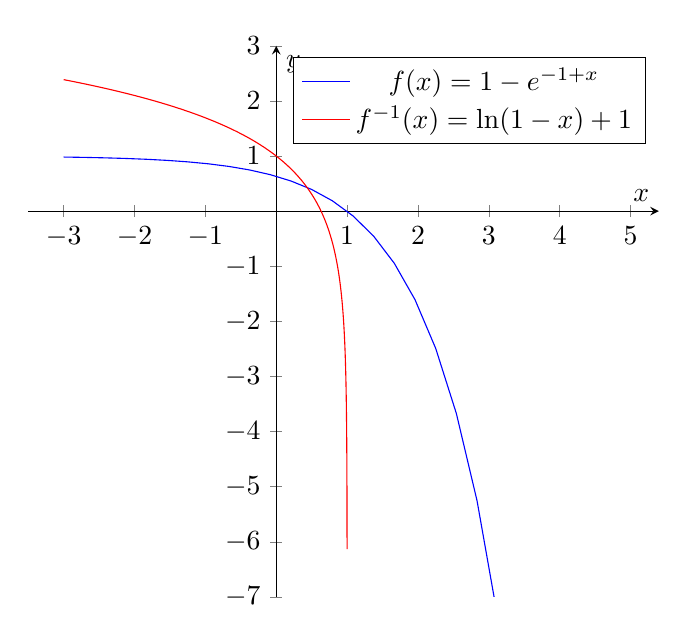
\begin{tikzpicture}
\begin{axis}[
x =.9 cm, y=.7 cm,
 axis lines=middle,
  xmin=-3.5,xmax=5.4,ymin=-7,ymax=3,
  xtick distance=1,
  ytick distance=1,
  xlabel=$x$,
  ylabel=$y$]
\addplot [blue,domain=-3:4] {1-exp(-1+x)};
\addlegendentry{\(f(x)=1-e^{-1+x}\)}
\addplot [red,domain=-3:1, samples=5000] {ln(1-x)+1};
\addlegendentry{\(f^{-1}(x)=\ln(1-x)+1\)}
\end{axis}
\end{tikzpicture}
		\end{center}
	\end{enumerate}
	\item Hitunglah $$ \int \dfrac{x^4+x^3+5x^2+2x+2}{x^3+x} \, dx $$
	\textbf{Solusi:}\\
	Tinjau bahwa 
	\begin{align*}
	x^4+x^3+5x^2+2x+2 &= x^4+x^2+x^3+4x^2+2x+2\\
	&= x(x^3+x)+(x^3+x)+4x^2+x+2\\
	&= (x^3+x)(x+1)+2x^2+2+2x^2+x\\
	&= (x^3+x)(x+1)+2(x^2+1)+x(2x+1)
	\end{align*}
	sehingga
	\begin{align*}
	\dfrac{x^4+x^3+5x^2+2x+2}{x^3+x} &= \dfrac{(x^3+x)(x+1)+2(x^2+1)+x(2x+1)}{x(x^2+1)}\\
	&= x+1 + \dfrac{2}{x} + \dfrac{2x+1}{x^2+1}\\
	&= x+1 + \dfrac{2}{x} + \dfrac{2x}{x^2+1} + \dfrac{1}{x^2+1}
	\end{align*}
	Jadi 
	\begin{align*}
	\int \dfrac{x^4+x^3+5x^2+2x+2}{x^3+x} \, dx &= \int x+1 + \dfrac{2}{x} + \dfrac{2x}{x^2+1} + \dfrac{1}{x^2+1} \, dx\\
	&= \dfrac{x^2}{2} + x +2\ln|x| +\ln|x^2+1| + \tan^{-1}(x) +C 
	\end{align*}
	\item Selesaikan integral berikut $$ \int_0^{\infty} \dfrac{e^{-\sqrt{x}}}{\sqrt{x}}\, dx $$
	\textbf{Solusi:}\\
	Misalkan $-\sqrt{x}=u$ sehingga $-\dfrac{1}{2\sqrt{x}}\, dx = du$ atau $\dfrac{1}{\sqrt{x}} \, dx = -2\, du$. Untuk $x=0$, maka $u=0$, dan untuk $x\rightarrow \infty$, maka $u \rightarrow-\infty$, sehingga diperoleh
	\begin{align*}
	\int_0^{\infty} \dfrac{e^{-\sqrt{x}}}{\sqrt{x}}\, dx &= \int_0^{-\infty} e^{u}(-2\, du)\\
	&= 2\int_{-\infty}^0 e^u \, du\\
	&= \lim_{a\rightarrow -\infty} 2\int_a^0 e^u \, du \\
	&= 2\cdot\lim_{a\rightarrow -\infty} e^u\bigg|^0_a \\
	&= 2\cdot\lim_{a\rightarrow -\infty} e^0-e^a \\
	&= 2\cdot\lim_{a\rightarrow -\infty} 1-e^a
	\end{align*}
	Tinjau bahwa $\displaystyle \lim_{a\rightarrow -\infty}e^a=0$ sehingga $$\int_0^{\infty} \dfrac{e^{-\sqrt{x}}}{\sqrt{x}}\, dx=2$$
	\item Misalkan $f$ dan $g$ fungsi-fungsi yang terdiferensial dengan 
	$a\neq 0.~b\neq 0,$ dan
	$$ \lim_{x\rightarrow +\infty} f(x) = +\infty, ~~\lim_{x\rightarrow +\infty} g(x) = +\infty, ~~\lim_{x\rightarrow +\infty} f'(x) = a,~~ \lim_{x\rightarrow +\infty} g'(x) = b $$
	Tentukan $\displaystyle \lim_{x\rightarrow +\infty} \dfrac{\ln f(x)}{\ln g(x)}=\cdots$\\
	\textbf{Solusi:}\\
	Karena merupakan bentuk tak tentu, maka dengan aturan L'hopital, dapat diperoleh
	\begin{align*}
	\lim_{x\rightarrow +\infty} \dfrac{\ln f(x)}{\ln g(x)} &= \lim_{x\rightarrow +\infty} \dfrac{f'(x)/f(x)}{g'(x)/g(x)} \\
	&= \lim_{x\rightarrow +\infty} \dfrac{f'(x)g(x)}{g'(x)f(x)}\\
	&= \lim_{x\rightarrow +\infty} \dfrac{f'(x)}{g'(x)}\times \lim_{x\rightarrow +\infty} \dfrac{g(x)}{f(x)} \\
	&= \dfrac{a}{b}\times \lim_{x\rightarrow +\infty} \dfrac{g'(x)}{f'(x)}\\
	&= \dfrac{a}{b}\times \dfrac{b}{a}\\
	&= 1
	\end{align*}
	\item Diberikan bidang datar yang dibatasi kurva: $y=\sqrt{x-1}$ dan $x-2y=1$ jika diputar menurut garis $x=\dfrac{1}{2}$. Sketsalah dan tentukan volume benda putar yang terjadi!\\
	\textbf{Solusi:}\\
	\textbf{Metode Cakram}\\
	Tinjau bahwa $x=1+2y$ sehingga $y=\sqrt{2y}$, diperoleh $y^2=2y$, maka $y=0$ atau $y=2$. Untuk $y=0$, maka $x=1$ dan untuk $y=2$, maka $x=5$. Diperoleh titik potongnya adalah $(1,0)$ dan $(5,2)$. Berikut sketsa grafiknya (benda putarnya gambar sendiri hehe :D) 
	\begin{center}
		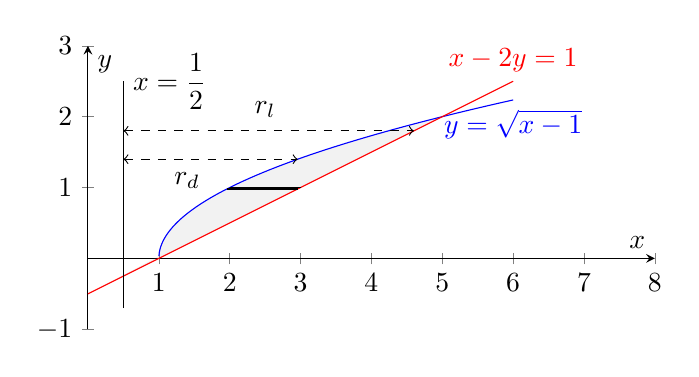
\begin{tikzpicture}
\begin{axis}[
x =.9 cm, y=.9 cm,
 axis lines=middle,
  xmin=0,xmax=8,ymin=-1,ymax=3,
  xtick distance=1,
  ytick distance=1,
  xlabel=$x$,
  ylabel=$y$]
\addplot [blue,domain=0:5, samples=1000, name path=B] {sqrt(x-1)};
\addplot [blue,domain=5:6, samples=1000] {sqrt(x-1)} node [below] {$y=\sqrt{x-1}$};
\addplot [red,domain=0:5, name path=A] {(x-1)/2};
\addplot [red,domain=5:6] {(x-1)/2} node [above] {$x-2y=1$};
\addplot[gray,opacity=0.1] fill between[of=B and A];
\draw (0.5,-0.7) -- (0.5,2.5) node [right] {$x=\dfrac{1}{2}$};
\draw (2,1) -- (3,1);
\draw (1.999,0.999) -- (2.999,0.999);
\draw (2.96,0.98) -- (1.9604,0.98);
\draw[<->,dashed] (0.5,1.4) -- (1.4*1.4+1,1.4);
\draw (1.4,1.1) node {$r_d$};
\draw[<->,dashed] (0.5,1.8) -- (1+2*1.8,1.8);
\draw (2.5,2.1) node {$r_l$};
\end{axis}
\end{tikzpicture}
		\end{center}
	Perhatikan bahwa $x=y^2+1,y\geq 0$ dan $x=1+2y$. \\Jari-jari dalamnya adalah $r_d=y^2+1-\dfrac{1}{2}$ dan jari-jari luar adalah $r_l=1+2y-\dfrac{1}{2}$.\\
	Perhatikan bahwa batasnya adalah dari $y=0$ hingga $y=2$, maka 
	\begin{align*}
	V =\pi \int_a^b r_l^2-r_d^2\, dy &= \pi\int_0^2 \left(2y+\dfrac{1}{2}\right)^2-\left( y^2+\dfrac{1}{2}\right)^2\, dy\\
	&= \pi \int_0^2 4y^2+2y+\dfrac{1}{4}-y^4-y^2-\dfrac{1}{4}\, dy\\
	&= \pi\int_0^2 -y^4+3y^2+2y\, dy\\
	&= \pi\left[-\dfrac{y^5}{5}+y^3+y^2\right]^2_0\\
	&= \pi \left[-\dfrac{32}{5}+8+4\right] \\
	&= \dfrac{28}{5}\pi
	\end{align*}
	\textbf{Metode Cincin Silinder}\\
	Tinjau bahwa jari-jarinya adalah $r=x-\dfrac{1}{2}$, sedangkan tingginya $h=\sqrt{x-1}-\dfrac{x-1}{2}$
	\begin{center}
		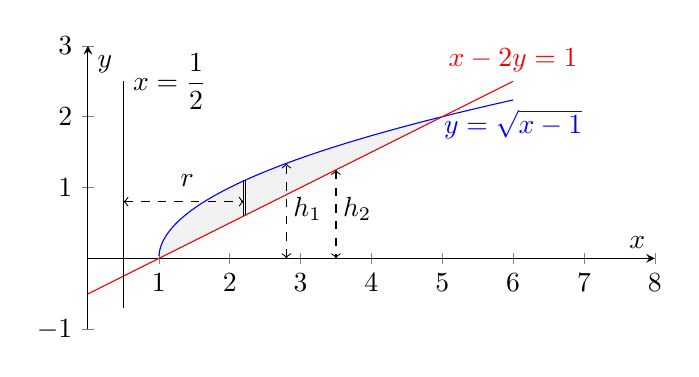
\begin{tikzpicture}
\begin{axis}[
x =.9 cm, y=.9 cm,
 axis lines=middle,
  xmin=0,xmax=8,ymin=-1,ymax=3,
  xtick distance=1,
  ytick distance=1,
  xlabel=$x$,
  ylabel=$y$]
\addplot [blue,domain=0:5, samples=1000, name path=B] {sqrt(x-1)};
\addplot [blue,domain=5:6, samples=1000] {sqrt(x-1)} node [below] {$y=\sqrt{x-1}$};
\addplot [red,domain=0:5, name path=A] {(x-1)/2};
\addplot [red,domain=5:6] {(x-1)/2} node [above] {$x-2y=1$};
\addplot[gray,opacity=0.1] fill between[of=B and A];
\draw (0.5,-0.7) -- (0.5,2.5) node [right] {$x=\dfrac{1}{2}$};
\draw (2.222,1.111-0.5) -- (2.222,1.10544109);
\draw (2.2,1.1-0.5) -- (2.2,1.109545);
\draw (2.220,1.110-0.5)--(2.220,1.1045361);
\draw[<->,dashed] (0.5,0.8) -- (2.2,0.8);
\draw (1.4,1.1) node {$r$};
\draw[dashed,<->] (2.8,0) -- (2.8,1.34164079);
\draw (3.1,0.7) node {$h_1$};
\draw[dashed,<->] (3.5,1.25) -- (3.5,0);
\draw (3.8,0.7) node {$h_2$};
\end{axis}
\end{tikzpicture}
		\end{center}
		Perhatikan bahwa batasnya adalah dari $x=1$ hingga $x=5$, diperoleh 
		\begin{align*}
		V = 2\pi \int_a^b rh\, dx &= 2\pi \int_1^5 \left(x-\dfrac{1}{2}\right)\left(\sqrt{x-1}-\dfrac{x-1}{2}\right)\, dx
		\end{align*}
		Misalkan $x-1=u$ sehingga $x=u+1$ dan $du=dx$. Untuk $x=1$, maka $u=0$, dan untuk $x=5$, maka $u=4$, diperoleh
		\begin{align*}
		V &= 2\pi \int_0^4 \left(u+1-\dfrac{1}{2}\right)\left(\sqrt{u}-\dfrac{u}{2}\right)\, du\\
		&= 2\pi\int_0^4 u\sqrt{u}+\dfrac{1}{2}\sqrt{u}-\dfrac{u^2}{2}-\dfrac{u}{4}\, du\\
		&= 2\pi \left[\dfrac{2u^2\sqrt{u}}{5}+\dfrac{u\sqrt{u}}{3}-\dfrac{u^3}{6}-\dfrac{u^2}{8}\right]^4_0\\
		&= 2\pi \left[\dfrac{2(4)^2\sqrt{4}}{5}+\dfrac{4\sqrt{4}}{3}-\dfrac{4^3}{6}-\dfrac{4^2}{8}\right]\\
		&= \dfrac{28}{5}\pi
		\end{align*}
		Jadi volume benda putar yang terjadi adalah $V=\dfrac{28}{5}\pi$
\end{enumerate}
\newpage
\section*{SOAL KELAS 10-18}
\begin{enumerate}
	\item Temperatur air yang dimasak di dalam ketel dimodelkan dalam bentuk $T=75e^{-kt}+22$ di mana $T$ adalah temperatur air $t$ menit setelah kompor dimatikan, dan $k$ adalah konstanta positif.
	\begin{enumerate}
		\item Tentukan tingkat perubahan temperatur dalam bentuk $k$.
		\item Setelah 5 menit, temperatur air adalah $70^\circ C$. Tentukan nilai $k$. Tuliskan jawaban dalam bentuk logaritma natural.
		\item Berapa menit waktu yang dibutuhkan agar temperature air menjadi lebih dingin ke $55^\circ C$? Tuliskan jawaban dalam bentuk logaritma natural
	\end{enumerate}
	\textbf{Solusi:}
	\begin{enumerate}
		\item Nyatakan $k$ dalam fungsi $T$ dan $t$
		\begin{align*}
		T-22 &= 75e^{-kt}\\
		\dfrac{T-22}{75} &= e^{-kt}\\
		\ln\left(\dfrac{T-22}{75}\right) &= \ln(e^{-kt})\\
		\ln\left(\dfrac{T-22}{75}\right) &= -kt\\
		k &= -\dfrac{1}{t}\ln\left(\dfrac{T-22}{75}\right)
		\end{align*}
		\item Dalam 5 menit temperatur air menjadi $70^\circ C$ sehingga
		\begin{align*}
		k &= -\dfrac{1}{5}\ln\left(\dfrac{70-22}{75}\right) \\
		&= -\dfrac{1}{5}\ln(0,64)
		\end{align*}
		\item Perhatikan bahwa $t=-\dfrac{1}{k}\ln\left(\dfrac{T-22}{75}\right)$ sehingga
		\begin{align*}
		t &= -\dfrac{1}{-\dfrac{1}{5}\ln(0,64)}\ln\left(\dfrac{55-20}{75}\right)\\
		&= \dfrac{5\ln(0,47)}{\ln(0,64)}
		\end{align*}
	\end{enumerate}
	\newpage
	\item Selesaian integral berikut ini:
	\begin{enumerate}
		\item $\displaystyle \int x\ln^2 x\, dx$
		\item $\displaystyle \int \dfrac{dx}{x^2+6x+12}$
	\end{enumerate}
	\textbf{Solusi:}
	\begin{enumerate}
		\item Misalkan $x=e^p$ sehingga $dx = e^p \, dp$, maka
	\begin{align*}
	\int x\ln^2 x\, dx &= \int e^{2p}\ln^2(e^p)\, dp\\
	&= \int p^2e^{2p} \, dp
	\end{align*}
	Misalkan $p^2=u$ sehingga $2p\, dp = du$, dan $e^{2p}\, dp = dv$ sehingga $v=\dfrac{e^{2p}}{2}$, maka dengan integral parsial diperoleh
	\begin{align*}
	\int x\ln^2 x\, dx &= \dfrac{p^2e^{2p}}{2} - \int \dfrac{2pe^{2p}}{2}\, dp\\
	&= \dfrac{p^2e^{2p}}{2}-\int pe^{2p}\, dp
	\end{align*}
	Misalkan pula $p=u$ dan $e^{2p}\, dp = dv$ sehingga $dp=du$ dan $v=\dfrac{e^{2p}}{2}$, diperoleh 
	\begin{align*}
	\int x\ln^2 x\, dx &= \dfrac{p^2e^{2p}}{2}-\int pe^{2p}\, dp\\
	&= \dfrac{p^2e^{2p}}{2} - \left(\dfrac{pe^{2p}}{2}-\int \dfrac{e^{2p}}{2}\, dp\right)\\
	&= \dfrac{p^2e^{2p}-pe^{2p}}{2}+\dfrac{e^{2p}}{4} + C\\
	&= e^{2p}\left(\dfrac{2p^2-2p+1}{4}\right) +C\\
	&= x^2\left(\dfrac{2\ln^2x-2\ln x+1}{4}\right) +C
	\end{align*}
	\item Tinjau bahwa $x^2+6x+12=(x+3)^2+3$. \\Misalkan $x+3=\sqrt{3}u$ sehingga $dx=\sqrt{3}\, du$, maka
	\begin{align*}
	\int \dfrac{dx}{x^2+6x+12} &= \dfrac{1}{(x+3)^2+3}\, dx\\
	&= \int \dfrac{\sqrt{3}}{3u^2+3}\,du\\
	&= \dfrac{\sqrt{3}}{3}\int \dfrac{1}{u^2+1}\, du\\
	&= \dfrac{\sqrt{3}}{3}\tan^{-1}(u) +C\\
	&= \dfrac{\sqrt{3}}{3}\tan^{-1}\left(\dfrac{x+3}{\sqrt{3}}\right) +C
	\end{align*}
	\end{enumerate}
	\newpage
	\item Hitunglah $\displaystyle \lim_{x\rightarrow \infty} (3^x+5^x)^\frac{1}{x}$\\
	\textbf{Solusi:}\\
	\textbf{CARA I}\\
	Tinjau bahwa $(3^x+5^x)^{\frac{1}{x}}=e^{\ln(3^x+5^x)^{\frac{1}{x}}}$. Cari terlebih dahulu $\displaystyle \lim_{x\rightarrow \infty} \ln(3^x+5^x)^\frac{1}{x}$
	\begin{align*}
	\lim_{x\rightarrow \infty} \ln(3^x+5^x)^\frac{1}{x} &= \lim_{x\rightarrow \infty} \dfrac{\ln\left(\dfrac{3^x+5^x}{5^x}\times 5^x\right)}{x}\\
	&= \lim_{x\rightarrow \infty} \dfrac{\ln\left(\left(\dfrac{3}{5}\right)^x+1\right)+\ln 5^x}{x}
	\end{align*}
	Tinjau bahwa $\lim_{x\rightarrow \infty} \left(\dfrac{3}{5}\right)^x=0$ karena $0<\dfrac{3}{5}<1$, maka
	\begin{align*}
	\lim_{x\rightarrow \infty} \ln(3^x+5^x)^\frac{1}{x} &= \lim_{x\rightarrow \infty} \dfrac{\ln(0+1)+x\ln 5}{x} \\
	&= \lim_{x\rightarrow \infty} \dfrac{x\ln 5}{x}\\
	&= \lim_{x\rightarrow \infty} \ln 5\\
	&= \ln 5
	\end{align*}
	Jadi 
	$$ \lim_{x\rightarrow \infty} (3^x+5^x)^{\frac{1}{x}} = \lim_{x\rightarrow \infty} e^{\ln(3^x+5^x)^\frac{1}{x}} = e^{\ln 5} = 5$$
	\textbf{CARA II}\\
	Tinjau bahwa $5^x\leq3^x+5^x\leq 2\cdot 5^x$ sehingga $5\leq(3^x+5^x)^{\frac{1}{x}}\leq 2^{\frac{1}{x}}\cdot 5$, maka
	\begin{align*}
	\lim_{x\rightarrow \infty} 5&\leq\lim_{x\rightarrow \infty} (3^x+5^x)^{\frac{1}{x}}\leq\lim_{x\rightarrow \infty} 5\cdot 2^{\frac{1}{x}}\\
	5&\leq\lim_{x\rightarrow \infty} (3^x+5^x)^{\frac{1}{x}}\leq 5
	\end{align*}
	Berdasarkan teorema apit, diperoleh
	$$\lim_{x\rightarrow \infty} (3^x+5^x)^{\frac{1}{x}} = 5 $$
	\item Tentukan luas daerah yang dibatasi oleh $y=2+|x-1|$ dan $y=-\dfrac{1}{5}x+7$, serta sketsalah grafiknya.\\
	\textbf{Solusi:}\\
	Tinjau bahwa untuk $y=2+|x-1|$ adalah fungsi nilai mutlak yang digeser ke kanan 1 satuan dan ke atas 2 satuan. Sedangkan $y=-\dfrac{1}{5}x+7$ adalah persamaan garis dengan gradien $-\dfrac{1}{5}$. Untuk mencari titik potongnya, tinjau $|x-1|=\begin{cases}x-1, ~ &x\geq 1\\
		-x+1, ~&x<1\end{cases}$, sehingga untuk $x\geq 1$
		\begin{align*}
		2+x-1 &= -\dfrac{1}{5}x+7\\
		\dfrac{6}{5}x &=6\\
		x &= 5
		\end{align*}
		Karena $x=5$, maka $y=2+|5-1|=6$. Untuk $x<1$ 
		\begin{align*}
		2-x+1 &= -\dfrac{1}{5}x+7\\
		\dfrac{4}{5}x &= -4\\
		x &= -5
		\end{align*}
		Karena $x=-5$, maka $y=2+|-5-1|=8$. Diperoleh titik potongnya adalah $(-5,8)$ dan $(5,6)$. Untuk grafiknya, dapat kita potong menjadi dua bagian sebagai berikut
	\begin{center}
		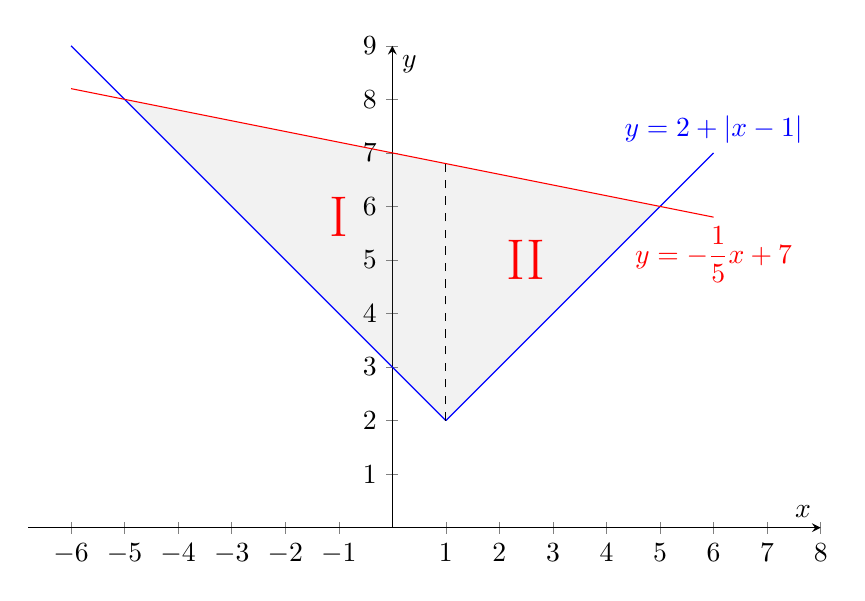
\begin{tikzpicture}
\begin{axis}[
x =.68 cm, y=.68 cm,
 axis lines=middle,
  xmin=-6.8,xmax=8,ymin=0,ymax=9,
  xtick distance=1,
  ytick distance=1,
  xlabel=$x$,
  ylabel=$y$]
\addplot [blue,domain=-5:5, samples=1000, name path=B] {2+abs(x-1)};
\addplot [blue,domain=5:6, samples=1000] {2+abs(x-1)} node [above] {$y=2+|x-1|$};
\addplot [blue,domain=-6:-5, samples=1000] {2+abs(x-1)};
\addplot [red,domain=-5:5, name path=A] {-0.2*x+7};
\addplot [red,domain=5:6, samples=1000] {-0.2*x+7} node [below] {$y=-\dfrac{1}{5}x+7$};
\addplot [red,domain=-6:-5] {-0.2*x+7};
\draw[dashed] (1,2) -- (1,7-0.2);
\addplot[gray,opacity=0.1] fill between[of=B and A];
\draw[red] (-1,5.8) node {\huge{I}};
\draw[red] (2.5,5) node {\huge{II}};
\end{axis}
\end{tikzpicture}
		\end{center}
		Untuk daerah I, luasnya adalah $\displaystyle \int_{-5}^1 -\dfrac{1}{5}x+7-(2-x+1)\, dx$. Sedangkan daerah II, luasnya adalah $\displaystyle \int_1^5 -\dfrac{1}{5}x+7-(2+x-1)\, dx$ sehingga luas totalnya adalah 
		\begin{align*}
		L &= \int_{-5}^1 -\dfrac{1}{5}x+7-(2-x+1)\, dx + \int_1^5 -\dfrac{1}{5}x+7-(2+x-1)\, dx\\
		&= \int_{-5}^1 \dfrac{4}{5}x+4\, dx + \int_1^5 -\dfrac{6}{5}x+6\, dx\\
		&= \dfrac{2}{5}x^2+4x\bigg|^1_{-5} - \dfrac{3}{5}x^2+6x\bigg|^5_1\\
		&= \left(\dfrac{2}{5}+4\right)-(10-20)+(-15+30)-\left(-\dfrac{3}{5}+6\right)\\
		&= 24
		\end{align*}
		\item Sketsa dataran yang dibatasi oleh $y=4-2x, ~y=4-x^2$, selanjutnya tentukan volume benda putar jika dataran tersebut diputar terhadap garis $x=3$.\\
		\textbf{Solusi:}\\
		\textbf{Metode Cakram}\\
		Tinjau titik potongnya, yaitu 
		\begin{align*}
		4-2x &= 4-x^2\\
		x^2-2x &= 0\\
		x(x-2) &=0
		\end{align*}
		Untuk $x=0$ diperoleh $y=4$, dan untuk $x=2$, diperoleh $y=0$, sehingga titik potongnya adalah $(0,4)$ dan $(2,0)$. Berikut grafiknya
		\begin{center}
		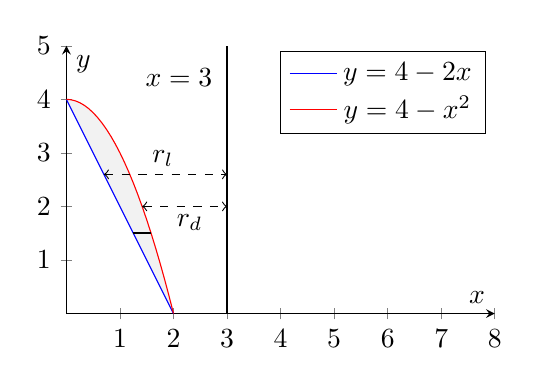
\begin{tikzpicture}
\begin{axis}[
x =.68 cm, y=.68 cm,
 axis lines=middle,
  xmin=0,xmax=8,ymin=0,ymax=5,
  xtick distance=1,
  ytick distance=1,
  xlabel=$x$,
  ylabel=$y$]
\addplot [blue,domain=0:2, samples=1000, name path=B] {4-2*x};
\addlegendentry{\(y=4-2x\)}
\addplot [red,domain=0:2, name path=A] {4-x^2};
\addlegendentry{\(y=4-x^2\)}
\addplot[gray,opacity=0.1] fill between[of=B and A];
\draw (3,0) -- (3,5);
\draw (1.25,1.5) -- (1.58114,1.5);
\draw (1.5843,1.49) -- (1.255,1.49);
\draw (1.245,1.51) -- (1.57797,1.51);
\draw[<->,dashed] (1.41421,2) -- (3,2);
\draw (2.3,1.7) node {$r_d$};
\draw[<->,dashed] (0.7,2.6) -- (3,2.6);
\draw (1.8,2.9) node {$r_l$};
\draw (2.1,4.4) node {$x=3$};
\end{axis}
\end{tikzpicture}
		\end{center}
		Perhatikan bahwa untuk $x\geq 0$, $x=\sqrt{4-y}$ dan $x=\dfrac{4-y}{2}$. \\
		Jari-jari dalamnya $r_d=3-\sqrt{4-y}$, sedangkan jari-jari luarnya $r_l=3-\dfrac{4-y}{2}=\dfrac{y+2}{2}$.\\
		Perhatikan bahwa batasnya adalah dari $y=0$ hingga $y=4$, maka
		\begin{align*}
		V =\pi \int_a^b r_l^2-r_d^2\, dy &= \pi\int_0^4 \left(\dfrac{y+2}{2}\right)^2-(3-\sqrt{4-y})^2\, dy\\
		&= \pi \int_0^4 \dfrac{y^2+4y+4}{4}-(9-6\sqrt{4-y}+4-y)\, dy\\
		&= \pi \int_0^4 \dfrac{y^2}{4}+2y-12+6\sqrt{4-y}\, dy\\
		&= \pi \left[\dfrac{y^3}{12}+y^2-12y-4(4-y)\sqrt{4-y}\right]^4_0\\
		&= \pi \left[\left(\dfrac{16}{3}+16-48-0-\left(-4(4)\sqrt{4}\right)\right)\right]\\
		&= \dfrac{16}{3}\pi
		\end{align*}
		\newpage
		\textbf{Metode Cincin Silinder}\\
		Tinjau bahwa jari-jarinya adalah $r=3-x$, sedangkan tingginya $h=4-x^2-(4-2x)=2x-x^2$
		\begin{center}
		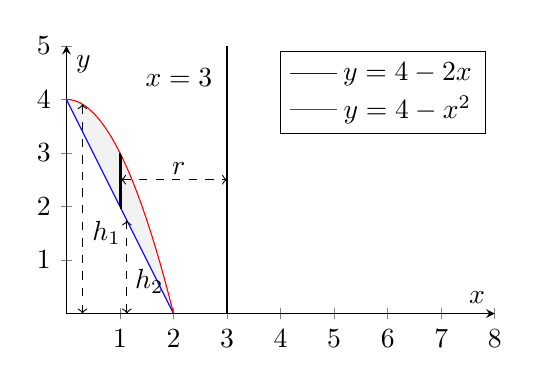
\begin{tikzpicture}
\begin{axis}[
x =.68 cm, y=.68 cm,
 axis lines=middle,
  xmin=0,xmax=8,ymin=0,ymax=5,
  xtick distance=1,
  ytick distance=1,
  xlabel=$x$,
  ylabel=$y$]
\addplot [blue,domain=0:2, samples=1000, name path=B] {4-2*x};
\addlegendentry{\(y=4-2x\)}
\addplot [red,domain=0:2, name path=A] {4-x^2};
\addlegendentry{\(y=4-x^2\)}
\addplot[gray,opacity=0.1] fill between[of=B and A];
\draw (3,0) -- (3,5);
\draw[<->,dashed] (0.3,3.91) -- (.3,0);
\draw (0.75,1.5) node {$h_1$};
\draw[<->,dashed] (1.13,0) -- (1.13,4-2*1.13);
\draw (1.55,0.6) node {$h_2$};
\draw (2.1,4.4) node {$x=3$};
\draw (1,2) -- (1,3);
\draw (1.02,4-2*1.02) -- (1.02,4-1.02^2);
\draw[dashed,<->] (1.02,2.5) -- (3,2.5);
\draw (2.1,2.7) node {$r$};
\end{axis}
\end{tikzpicture}
		\end{center}
		Perhatikan bahwa batasnya adalah dari $x=0$ hingga $x=2$, diperoleh 
		\begin{align*}
		V = 2\pi \int_a^b rh\, dx &= 2\pi \int_0^2 (3-x)(2x-x^2)\, dx\\
		&= 2\pi\int_0^2 6x-5x^2+x^3\, dx\\
		&= 2\pi\left[3x^2-\dfrac{5}{3}x^3+\dfrac{x^4}{4}\right]\\
		&= 2\pi \left[3(2)^2-\dfrac{5(2)^3}{3}+\dfrac{2^4}{4}\right]\\
		&= \dfrac{16}{3}\pi
		\end{align*}
		Jadi volume benda putar tersebut adalah $V=\dfrac{16}{3}\pi$
\end{enumerate}
\newpage
\section*{SOAL KELAS 19-27}
\begin{enumerate}
	\item Diberikan fungsi $f$ dengan $f(x)=x^7+6x^5+4x^3+x+1$.
	\begin{enumerate}
		\item Tunjukkan bahwa $f^{-1}$ diferensiabel pada selang $(-\infty,+\infty)$
		\item Misalkan $y=f^{-1}(x)$. Dapatkan turunan dari $f^{-1}$ dengan terlebih dahulu menghitung $\dfrac{dx}{dy}$
		\item Dapatkan turunan dari $f^{-1}$ dengan menggunakan diferensiasi implisit.
	\end{enumerate}
	\textbf{Solusi:}
	\begin{enumerate}
		\item Untuk menunjukkan bahwa $f^{-1}$ diferensiabel pada suatu selang, cukup kita tunjukkan bahwa turunan dari $f(x)$ tak nol untuk setiap $x$ pada selang tersebut. Tinjau bahwa $f'(x)=7x^6+30x^4+12x^2+1>0$ untuk setiap $x$ pada selang $(-\infty,+\infty)$ sehingga $f^{-1}$ diferensiabel pada selang tersebut.
		\item Misalkan $y=f^{-1}(x)$ sehingga $x=f(y)=y^7+6y^5+4y^3+y+1$ dan diperoleh 
		\begin{align*}
		\dfrac{dx}{dy} &= 7y^6+30y^4+12y^2+1\\
		\dfrac{dy}{dx} = \dfrac{1}{dx/dy} &= \dfrac{1}{7y^6+30y^4+12y^2+1}
\end{align*}		
	\item  Misalkan $y=f^{-1}(x)$ sehingga $x=f(y)=y^7+6y^5+4y^3+y+1$ dan diperoleh 
	\begin{align*}
	\dfrac{d}{dx}[x] &= \dfrac{d}{dx}[y^7+6y^5+4y^3+y+1]\\
	1 &= 7y^6\dfrac{dy}{dx}+30y^4\dfrac{dy}{dx}+12y^2\dfrac{dy}{dx}+\dfrac{dy}{dx}\\
	1 &= (7y^6+30y^4+12y^2+1)\dfrac{dy}{dx}\\
	\dfrac{dy}{dx} &= \dfrac{1}{7y^6+30y^4+12y^2+1}
	\end{align*}
	\end{enumerate}
	\item Selesaikan $$ \int \dfrac{\sqrt{2+x^2}}{x}\, dx$$
	\textbf{Solusi:}\\
	\textbf{CARA I}\\
	Misalkan $x=\sqrt{2}\tan u$ sehingga $dx = \sqrt{2}\sec^2 u$, maka
	\begin{align*}
	\int \dfrac{\sqrt{2+x^2}}{x}\, dx &= \int \dfrac{\sqrt{2}\sec^2 u\sqrt{2(1+\tan^2 u)}}{\sqrt{2}\tan u}\, du\\
	&= \sqrt{2}\int \dfrac{\sec^3 u}{\tan u}\, du\\
	&= \sqrt{2}\int \csc u\sec^2 u\, du\\
	&= \sqrt{2}\int \csc u(1+\tan^2u)\, du\\
	&= \sqrt{2}\int \csc u+\tan u\sec u\, du
	\end{align*}
	Ingat bahwa $\dfrac{d}{dx}\sec x = \tan x\sec x$ sehingga $\displaystyle \int \tan u \sec u\, du=\sec u$, diperoleh
	\begin{align*}
	\int \csc u+\tan u\sec u\, du &= \int \csc u\times \dfrac{\csc u+\cot u}{\csc u +\cot u}\, du +\sec u\\
	&= \sec u+ \int \dfrac{\csc^2 u+\csc u\cot u}{\csc u+\cot u} \, du
	\end{align*}
	Misalkan $p=\csc u+\cot u$ sehingga $dp = -\csc u\cot u-\csc^2u=-(\csc^2 u+\csc u\cot u) \, du$, maka
	\begin{align*}
	\int \dfrac{\csc^2 u+\csc u\cot u}{\csc u+\cot u} \, du &= \int -\dfrac{1}{p}\, dp\\
	&= -\ln|p| \\
	&= -\ln|\csc u+\cot u|
	\end{align*}
	Karena $x=\sqrt{2}\tan u$, maka $u=\tan^{-1}\left(\dfrac{x}{\sqrt{2}}\right)$. 
	\begin{center}
	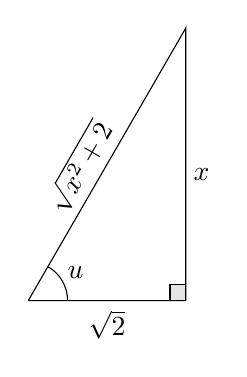
\begin{tikzpicture}
	\path (0,0) coordinate (A) (2*1,0) coordinate (B) (2*1,2*1.73) coordinate (C);
	\draw (1,0) node[below] {$\sqrt{2}$};
	\draw (0.6,0.36) node {$u$};
	\draw (2.2,1.6) node {$x$};
	\draw (A) -- (B) -- (C) -- (A);
	\draw (0:.5) arc (0:60:0.5);
	\node [rotate=60] at (0.65,1.7) {$\sqrt{x^2+2}$};
	\draw[fill=gray!20] (1.8,0) -- (1.8,0.2) -- (2,0.2) -- (2,0) -- (1.8,0);
	\end{tikzpicture}
\end{center}	
Diperoleh 
\begin{align*}
\sec u = \dfrac{\sqrt{x^2+2}}{\sqrt{2}}\qquad\qquad
\csc u = \dfrac{\sqrt{x^2+2}}{x} \qquad \qquad\cot u = \dfrac{\sqrt{2}}{x}
\end{align*}
Jadi 
\begin{align*}
\int \dfrac{\sqrt{2+x^2}}{x}\, dx &=\sqrt{2}\int \csc u+\tan u\sec u\, du\\ 
&= \sqrt{2}(\sec u-\ln|\csc u+\cot u|)+C\\
&= \sqrt{x^2+2}-\sqrt{2}\ln\left|\dfrac{\sqrt{x^2+2}}{x}+\dfrac{\sqrt{2}}{x}\right|+C
\end{align*}
\textbf{CARA II}\\
Tinjau bahwa $$\dfrac{\sqrt{x^2+2}}{x}=\dfrac{x^2+2}{x\sqrt{x^2+2}}=\dfrac{x}{\sqrt{x^2+2}}+\dfrac{2}{x\sqrt{x^2+2}}$$
sehingga
\begin{align*}
\int \dfrac{\sqrt{2+x^2}}{x}\, dx &= \int \dfrac{x}{\sqrt{x^2+2}}+\dfrac{2}{x\sqrt{x^2+2}}\, dx
\end{align*}
\begin{enumerate}[(i)]
	\item Untuk $\displaystyle  \int \dfrac{x}{\sqrt{x^2+2}}\, dx$. Misalkan $u=x^2+2$ sehingga $du = 2x\, dx$, maka
	\begin{align*}
	\int \dfrac{x}{\sqrt{x^2+2}}\, dx &= \int \dfrac{1}{2\sqrt{u}}\, du\\
	&= \sqrt{u}\\
	&= \sqrt{x^2+2}
\end{align*}	 
	\item Untuk $\displaystyle \int \dfrac{2}{x\sqrt{x^2+2}}\, dx$. Misalkan $x=\sqrt{2}u$ sehingga $dx=\sqrt{2} \, du$, maka
	\begin{align*}
	\int \dfrac{2}{x\sqrt{x^2+2}}\, dx &= \int \dfrac{2\sqrt{2}}{\sqrt{2}u\sqrt{2u^2+2}}\, du\\
	&= \int \dfrac{\sqrt{2}}{u\sqrt{u^2+1}}\, du\\
	&= -\sqrt{2}\csch^{-1}|u| \\
	&= -\sqrt{2}\csch^{-1}\left|\dfrac{x}{\sqrt{2}}\right|
	\end{align*}
	Jadi 
	\begin{align*}
\int \dfrac{\sqrt{2+x^2}}{x}\, dx &= \int \dfrac{x}{\sqrt{x^2+2}}\, dx+\int \dfrac{2}{x\sqrt{x^2+2}}\, dx\\
&= \sqrt{x^2+2}-\sqrt{2}\csch^{-1}\left|\dfrac{x}{\sqrt{2}}\right| +C 
\end{align*}
\textbf{Catatan:} Hasil kedua integral ekuivalen meski terlihat berbeda. \\Hasil lainnya
\begin{align*}
\int \dfrac{\sqrt{x^2+2}}{x}\, dx &= \sqrt{x^2+2}-\sqrt{2}\tanh^{-1}\left|\dfrac{\sqrt{x^2+2}}{\sqrt{2}}\right|+C\\
\int \dfrac{\sqrt{x^2+2}}{x}\, dx &= \sqrt{x^2+2}-\sqrt{2}\coth^{-1}\left|\dfrac{\sqrt{x^2+2}}{\sqrt{2}}\right|+C\\
\int \dfrac{\sqrt{x^2+2}}{x}\, dx &= \sqrt{x^2+2}-\dfrac{\sqrt{2}}{2}\left(\ln\left|\sqrt{\dfrac{x^2+2}{2}}+1\right|-\ln\left|\sqrt{\dfrac{x^2+2}{2}}-1\right|\right) +C\\
\int \dfrac{\sqrt{x^2+2}}{x}\, dx &= \sqrt{x^2+2}-\sqrt{2}\ln\left|\dfrac{\sqrt{x^2+2}}{x}-\dfrac{\sqrt{2}}{x}\right| +C\\
\int \dfrac{\sqrt{x^2+2}}{x}\, dx &= \sqrt{x^2+2}-\dfrac{1}{\sqrt{2}}\left(\ln|\sqrt{x^2+2}-\sqrt{2}|-\ln|\sqrt{x^2+2}+\sqrt{2}|\right) +C
\end{align*}
\newpage
\end{enumerate}
	\item Dapatkan nilai integral  $$\int_0^{\frac{\pi}{2}}\dfrac{\cos x}{\sqrt{1-\sin x}}\, dx $$
	\textbf{Solusi:}\\
	Misalkan $1-\sin x=u$ sehingga $-\cos x\, dx = du$. Untuk $x=0$, maka $u=1$, dan untuk $x=\dfrac{
	\pi}{2}$, maka $u=0$, diperoleh
	\begin{align*}
	\int_0^{\frac{\pi}{2}}\dfrac{\cos x}{\sqrt{1-\sin x}}\, dx &= \int_1^0 -\dfrac{du}{\sqrt{u}}\\
	&= \lim_{a\rightarrow 0^+}\int_a^1 u^{-\frac{1}{2}} \, du\\
	&= \lim_{a\rightarrow 0^+} 2u^\frac{1}{2}\bigg|^1_a\\
	&= \lim_{a\rightarrow 0^+} 2(1-\sqrt{a})=2
	\end{align*}
	\item Selesaikan $$ \int \dfrac{2x^2+3}{(x^2+1)^2}\, dx$$
	\textbf{Solusi:}\\
	Tinjau bahwa $2x^2+3=2(x^2+1)+1$ sehingga 
	\begin{align*}
	\int \dfrac{2x^2+3}{(x^2+1)^2}\, dx &= \int \dfrac{2(x^2+1)+1}{(x^2+1)^2}\, dx\\
	&= \int \dfrac{2}{x^2+1}\, dx+\int \dfrac{1}{(x^2+1)^2}\, dx
	\end{align*}
	Misalkan $x=\tan u$ sehingga $dx=\sec^2 u\, du$, diperoleh 
	\begin{align*}
	\int \dfrac{2x^2+3}{(x^2+1)^2}\, dx &= \int \dfrac{2\sec^2 u}{\tan^2 u+1}\, du + \int \dfrac{\sec^2 u}{(\tan^2 u + 1)^2} \, du\\
	&= \int \dfrac{2\sec^2 u}{\sec^2 u} \, du + \int \dfrac{\sec^2 u}{\sec^4 u}\, du\\	
	&= \int 2\, du + \int \cos^2 u\, du\\
	&= 2u + \dfrac{1}{2}\int 1+\cos 2u \, du\\
	&= 2u + \dfrac{1}{2}\left(u+\dfrac{1}{2}\sin 2u\right) +C
	\end{align*}
	Karena $x=\tan u$, maka $u=\tan^{-1}x$. 
	\begin{center}
	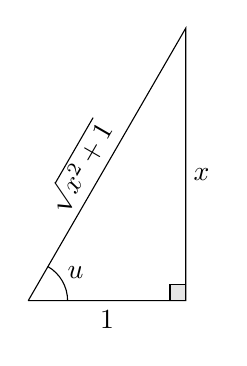
\begin{tikzpicture}
	\path (0,0) coordinate (A) (2*1,0) coordinate (B) (2*1,2*1.73) coordinate (C);
	\draw (1,0) node[below] {1};
	\draw (0.6,0.36) node {$u$};
	\draw (2.2,1.6) node {$x$};
	\draw (A) -- (B) -- (C) -- (A);
	\draw (0:.5) arc (0:60:0.5);
	\node [rotate=60] at (0.65,1.7) {$\sqrt{x^2+1}$};
	\draw[fill=gray!20] (1.8,0) -- (1.8,0.2) -- (2,0.2) -- (2,0) -- (1.8,0);
	\end{tikzpicture}
\end{center}		
	Diperoleh pula $\sin u=\dfrac{x}{\sqrt{x^2+1}}$ dan $\cos x=\dfrac{1}{\sqrt{x^2+1}}$ sehingga $$\sin 2u = 2\sin u\cos u =2\times\dfrac{x}{\sqrt{x^2+1}}\times \dfrac{1}{\sqrt{x^2+1}}=\dfrac{2x}{x^2+1}$$
	Jadi 
	\begin{align*}
	\int \dfrac{2x^2+3}{(x^2+1)^2}\, dx &= 2\tan^{-1} x +\dfrac{1}{2}\left(\tan^{-1} x +\dfrac{1}{2}\times\dfrac{2x}{x^2+1}\right)\\
	&= \dfrac{1}{2}\left(\dfrac{x}{x^2+1}+5\tan^{-1}x\right)+C
	\end{align*}
	\item Tentukan luas daerah yang dibatasi oleh kurva $y=|x|;y=-x^2+2$\\
	\textbf{Solusi:}\\
	Tinjau bahwa titik potongnya adalah $(-1,2)$ dan $(1,2)$
	\begin{center}
		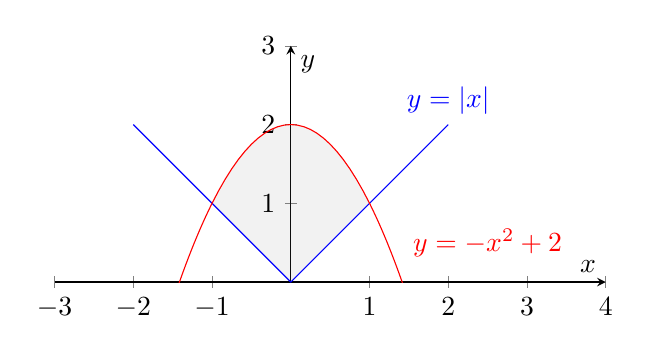
\begin{tikzpicture}
\begin{axis}[
x =1 cm, y=1 cm,
 axis lines=middle,
  xmin=-3,xmax=4,ymin=0,ymax=3,
  xtick distance=1,
  ytick distance=1,
  xlabel=$x$,
  ylabel=$y$]
\addplot [blue,domain=-1:1, samples=1000, name path=B] {abs(x)};
\addplot [blue,domain=1:2, samples=1000] {abs(x)} node [above] {$y=|x|$};
\addplot [blue,domain=-2:-1, samples=1000] {abs(x)};
\addplot [red,domain=-1:1, name path=A] {-x^2+2};
\addplot [red,domain=1:2] {-x^2+2};
\addplot [red,domain=-2:-1] {-x^2+2};
\draw[red] (2.5,0.5) node {$y=-x^2+2$};
\addplot[gray,opacity=0.1] fill between[of=B and A];
\end{axis}
\end{tikzpicture}
		\end{center}
		Untuk $x<0$, $|x|=-x$, sedangkan untuk $x\geq 0$, $|x|=x$ sehingga luasnya
		\begin{align*}
		L = \int_a^b f(x)-g(x) \, dx &=\int_{-1}^0 -x^2+2+x \, dx + \int_0^1 -x^2+2-x \, dx\\
		&= -\dfrac{x^3}{3}+2x+\dfrac{x^2}{2}\bigg|^0_{-1}  -\dfrac{x^3}{3}+2x-\dfrac{x^2}{2}\bigg|^1_0\\
		&= -\left(-\dfrac{(-1)^3}{3}+2(-1)+\dfrac{(-1)^2}{2}\right) -\dfrac{1}{3}+2-\dfrac{1}{2}\\
		&= \dfrac{7}{3}
		\end{align*}
\end{enumerate}
\newpage
\section*{SOAL KELAS 37-44}
\begin{enumerate}
	\item Jika $F(x)=f(2g(x))$, dengan $f(x)=x^4+x^3+1;0\leq x\leq 2$ dan $g(x)=f^{-1}(x)$. Dapatkan $F'(3)$\\
	\textbf{Solusi:}\\
	Kita punya $F'(x)=2f'(2g(x))g'(x)$, selanjutnya akan kita cari $g'(x)=(f^{-1})'(x)$. \\Misalkan $y=f^{-1}(x)$, maka $$ x=f(y)=y^4+y^3+1 $$
sehingga diperoleh
\begin{align*}
\dfrac{dx}{dy} &= 4y^3+3y^2\\
\dfrac{dy}{dx} = \dfrac{1}{dx/dy} &= \dfrac{1}{4y^3+3y^2}
\end{align*}
Perhatikan bahwa $g(3)=f^{-1}(3)$, dan ingat jika $y=f(x)$ maka $x=f^{-1}(y)$ sehingga $g(3)$ merupakan penyelesaian dari $x^4+x^3+1=3$. \\
Mudah terlihat bahwa $x=1$ memenuhi persamaan tersebut sehingga $g(3)=1$. \\
Ingat bahwa $g(x)=f^{-1}(x)=y$ sehingga $y=g(3)=1$ dan diperoleh 
$$ g'(3)=(f^{-1})'(3)=\dfrac{1}{4(1)^3+3(1)^2} = \dfrac{1}{7}$$ 
Substitusi semua yang telah diperoleh maka $$F'(3)=2f'(2g(3))g'(3) = \dfrac{2f'(2)}{7} $$
Dapat kita tentukan bahwa $f'(x)=4x^3+3x^2$ sehingga $f'(2)=4(2)^3+3(2)^2=44$ dan 
$$ F'(3) = \dfrac{2\times 44}{7} = \dfrac{88}{7} $$
	\item Dapatkan $\dfrac{dy}{dx}$ jika $y=\tan(\cos^{-1}x)$
	\\ \textbf{Solusi:}\\
	Ingat bahwa $\dfrac{d}{dx}\tan x=\sec^2 x$ dan $\dfrac{d}{dx} \cos^{-1}x=-\dfrac{1}{\sqrt{1-u^2}}$ serta aturan rantai, diperoleh
	\begin{align*}
	\dfrac{d}{dx}[\tan(\cos^{-1}x)] &= \sec^2(\cos^{-1}x)\dfrac{d}{dx}[\cos^{-1}x]\\
	&= \sec^2(\cos^{-1}x)\times \left(-\dfrac{1}{\sqrt{1-x^2}}\right)\\
	&= -\dfrac{1}{\cos^2(\cos^{-1}x)\sqrt{1-x^2}}\\
	&= -\dfrac{1}{x^2\sqrt{1-x^2}}
	\end{align*}
	\newpage
	\item Hitunglah $$ \int \dfrac{\sec^2\theta}{\tan^3\theta-\tan^2\theta}\, d\theta$$
	\textbf{Solusi:}\\
	Misalkan $x=\tan \theta$ sehingga $dx = \sec^2\theta\, d\theta$, diperoleh
	\begin{align*}
	\int \dfrac{\sec^2\theta}{\tan^3\theta-\tan^2\theta}\, d\theta &= \int \dfrac{1}{x^3-x^2}\, dx\\
	&= \int \dfrac{1}{x^2(x-1)}\, dx
	\end{align*}
	Tinjau dekomposisi pecahannya yaitu
	\begin{align*}
	\dfrac{1}{x^2(x-1)} &= \dfrac{A}{x} + \dfrac{B}{x^2} + \dfrac{C}{x-1}\\
	&= \dfrac{Ax+B}{x^2} + \dfrac{C}{x-1}\\
	&= \dfrac{(Ax+B)(x-1)+Cx^2}{x^2(x-1)}\\
	&= \dfrac{(A+C)x^2+(B-A)x-B}{x^2(x-1)}
	\end{align*}
	Diperoleh 
	\begin{align*}
	A+C &= 0\\
	B-A &= 0\\
	-B & = 1
	\end{align*}
	Jadi $A=-1, ~B=-1$ dan $C=1$ sehingga 
	\begin{align*}
	\int \dfrac{\sec^2\theta}{\tan^3\theta-\tan^2\theta}\, d\theta &= \int \dfrac{1}{x^2(x-1)}\, dx \\
	&= \int -\dfrac{1}{x} - \dfrac{1}{x^2} +\dfrac{1}{x-1} \, dx \\
	&= -\ln|x|+\dfrac{1}{x} +\ln|x-1|\\
	&= \dfrac{1}{\tan \theta} + \ln\left|\dfrac{\tan\theta -1}{\tan\theta}\right|\\
	&= \cot \theta +\ln|\cot\theta|+C
	\end{align*}
	\newpage
	\item Hitunglah $$ \int_{-\infty}^0 \dfrac{dx}{(2x-1)^3}$$
	\textbf{Solusi:}\\
	Misalkan $u=2x-1$ sehingga $du = 2\, dx$. Untuk $x=0$, maka $u=-1$ dan untuk $x\rightarrow -\infty$, maka $u\rightarrow -\infty$. Karena titik diskontinunya yaitu $x=\frac{1}{2}$ tidak di dalam interval batas integral, diperoleh  
	\begin{align*}
	\int_{-\infty}^0 \dfrac{dx}{(2x-1)^3} &= \int_{-\infty}^{-1} \dfrac{du}{2u^3}\\
	&= \lim_{a\rightarrow -\infty} \dfrac{1}{2}\int_a^{-1} \dfrac{du}{u^3}\\
	&= \lim_{a\rightarrow -\infty} \dfrac{1}{2}\left[-\dfrac{1}{2u^2}\right]^{-1}_a\\
	&= \lim_{a\rightarrow -\infty} \dfrac{1}{2}\left(-\dfrac{1}{2(-1)^2}-\left(-\dfrac{1}{2(a)^2}\right)\right)\\
	&= \lim_{a\rightarrow -\infty} \dfrac{1}{4}\left(\dfrac{1}{a^2}-1\right)\\
	&= \dfrac{1}{4}(0-1) = -\dfrac{1}{4}
	\end{align*}
	\item Gunakan metode cincin silinder untuk menentukan volume benda padat yang dibentuk oleh daerah dibatasi fungsi $f(x)=4-x$ dan sumbu-$x$ pada interval $x\in [0,4]$ dan diputar terhadap $y=-2$\\
	\textbf{Solusi:}\\
	Tinjau bahwa jari-jarinya adalah $r=y-(-2)=y+2$, sedangkan tingginya $h=4-y$
	\begin{center}
		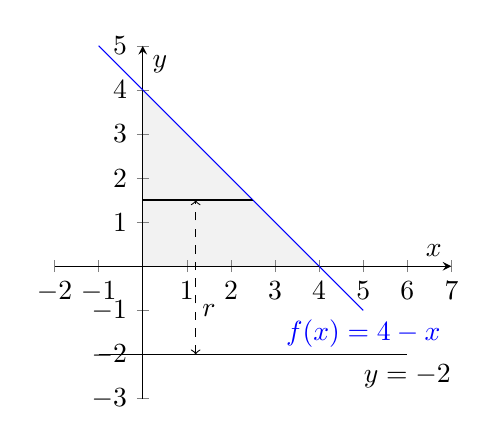
\begin{tikzpicture}
\begin{axis}[
x =.56 cm, y=.56 cm,
 axis lines=middle,
  xmin=-2,xmax=7,ymin=-3,ymax=5,
  xtick distance=1,
  ytick distance=1,
  xlabel=$x$,
  ylabel=$y$]
\addplot [blue,domain=0:4, samples=1000, name path=B] {4-x};
\addplot [blue,domain=4:5, samples=1000] {4-x} node [below] {$f(x)=4-x$};
\addplot [blue,domain=-1:0, samples=1000] {4-x};
\addplot [domain=0:4, name path=A] {0};
\addplot[gray,opacity=0.1] fill between[of=B and A];
\addplot [domain=-1:6] {-2} node [below] {$y=-2$};
\draw (0,1.5) -- (4-1.5,1.5);
\draw (0,1.52) -- (4-1.52,1.52);
\draw[dashed,<->] (1.2,-2) -- (1.2,1.5);
\draw (1.5,-1) node {$r$};
\end{axis}
\end{tikzpicture}
		\end{center}
		Batasnya adalah $y=0$ hingga $y=4$. Dengan metode cincin silinder diperoleh 
		\begin{align*}
		V = 2\pi \int_a^b rh\, dx &= 2\pi \int_0^4 (y+2)(4-y)\, dy\\
		&= 2\pi \int_0^4 -y^2+2y+8 \, dy\\
		&= 2\pi \left[-\dfrac{y^3}{3}+y^2+8y\right]^4_0\\
		&= 2\pi \left[-\dfrac{64}{3}+16+32\right] = \dfrac{160}{3}\pi
		\end{align*}
\end{enumerate}
\newpage
\section*{SOAL KELAS 45-52}
\begin{enumerate}
	\item Dapatkan turunan pertama dari $$ y= \dfrac{x^3\sqrt[5]{5x^2+12}}{(1+x^3)^4} $$
	\textbf{Solusi:}\\
	Bentuk tersebut terlihat cukup rumit, akan lebih mudah jika kita gunakan diferensiasi logaritmik, yaitu dengan mengoperasikan fungsi logaritma natural pada kedua ruas
	\begin{align*}
	\ln y &= \ln\left(\dfrac{x^3\sqrt[5]{5x^2+12}}{(1+x^3)^4}\right)\\
	\ln y &= \ln (x^3) +\ln (\sqrt[5]{5x^2+12}) -\ln((1+x^3)^4)\\
	\ln y &= 3\ln x+\dfrac{1}{5}\ln(5x^2+12)-4\ln(1+x^3)\\
	\dfrac{1}{y}\dfrac{dy}{dx} &= \dfrac{3}{x} + \dfrac{1}{5}\times \dfrac{1}{5x^2+12}\times 10x -\dfrac{4}{1+x^3}\times 3x^2\\
	\dfrac{1}{y}\dfrac{dy}{dx} &= \dfrac{3}{x} + \dfrac{2x}{5x^2+12}-\dfrac{12x^2}{1+x^3}\\
	\dfrac{dy}{dx} &= y\left[\dfrac{3}{x} + \dfrac{2x}{5x^2+12}-\dfrac{12x^2}{1+x^3}\right] \\
	\dfrac{dy}{dx} &= \left[\dfrac{x^3\sqrt[5]{5x^2+12}}{(1+x^3)^4}\right]\left[\dfrac{3}{x} + \dfrac{2x}{5x^2+12}-\dfrac{12x^2}{1+x^3}\right]
	\end{align*}
	\item Hitung integral berikut ini:
	\begin{enumerate}
		\item $$ \int \dfrac{2t-1}{t+t^{\frac{3}{5}}}\, dt $$
		\item $$ \int \dfrac{2x+1}{2x^3-x^2}\, dx$$
	\end{enumerate}
	\textbf{Solusi:}\\
	\begin{enumerate}
		\item Misalkan $t^\frac{1}{5}=u$ sehingga $\dfrac{1}{5t^{\frac{4}{5}}}\, dt = du$, dapat diperoleh
		\begin{align*}
		\dfrac{2t-1}{t+t^\frac{3}{5})}\, dt &= \dfrac{2t-1}{t^\frac{4}{5}(t^\frac{1}{5}+t^{-\frac{1}{5}}}\, dt\\
		&= \dfrac{5(2u^5-1)}{u+u^{-1}}\, du\\
		&= \dfrac{5(2u^6-u)}{u^2+1}\, du\\
		2u^6-u &= 2(u^6+u^4)-2u^4-u\\
		&= 2u^4(u^2+1)-2(u^4+u^2)+2u^2-u\\
		&= 2u^4(u^2+1) - 2u^2(u^2+1) + 2(u^2+1)-2 -u
		\end{align*}
		Bentuk integralnya menjadi
		\begin{align*}
		\int \dfrac{2t-1}{t+t^{\frac{3}{5}}}\, dt &= 5\int \dfrac{2u^4(u^2+1) - 2u^2(u^2+1) + 2(u^2+1)-2 -u}{u^2+1}\, du\\
		&= 5\int 2u^4-2u^2+2-\dfrac{u}{u^2+1} -\dfrac{2}{u^2+1}\, du\\
		&= 5\left[\dfrac{2}{5}u^5-\dfrac{2}{3}u^3+2u-\dfrac{1}{2}\ln(u^2+1)-2\tan^{-1}u\right] +C\\
		&= 2t - \dfrac{10}{3}t^\frac{3}{5}+10t^\frac{1}{5}-\dfrac{5}{2}\ln(t^{\frac{2}{5}}+1)-10\tan^{-1}t^\frac{1}{5} +C 
		\end{align*}
		\item Tinjau bahwa $2x^3-x^2=x^2(2x-1)$ sehingga dekomposisi pecahannya
		\begin{align*}
		\dfrac{2x+1}{2x^3-x^2} &= \dfrac{A}{x} + \dfrac{B}{x^2} + \dfrac{C}{2x-1} \\
		&= \dfrac{Ax+B}{x^2} + \dfrac{C}{2x-1}\\
		&= \dfrac{(Ax+B)(2x-1)+Cx^2}{x^2(2x-1)}\\
		&= \dfrac{(2A+C)x^2+(2B-A)x-B}{2x^3-x^2}
		\end{align*}
		Diperoleh
		\begin{align*}
		2A+C = 0 \qquad \text{dan}\qquad 2B-A=2 \qquad \text{dan}\qquad -B = 1
		\end{align*}
		Jadi $A=-4,B=-1,$ dan $C=8$, sehingga
		\begin{align*}
		\int \dfrac{2x+1}{2x^3-x^2}\, dx &= \int -\dfrac{4}{x} - \dfrac{1}{x^2} + \dfrac{8}{2x-1}\, dx\\
		&= -4\ln |x|+\dfrac{1}{x}+4\ln|2x-1| + C
		\end{align*}
	\end{enumerate}
	\item Selesaikan 
	$$ \int_0^4 \dfrac{dx}{\sqrt[3]{x-1}} $$
	\textbf{Solusi:}\\
	Karena titik diskotinunya, yaitu $x=1$ berada dalam interval batas integral, maka 
	\begin{align*}
	\int_0^4 \dfrac{dx}{\sqrt[3]{x-1}} = \int_0^1 \dfrac{dx}{\sqrt[3]{x-1}} + \int_1^4 \dfrac{dx}{\sqrt[3]{x-1}}
	\end{align*}
	Selanjutnya, hitung integral tak tentunya dahulu. Misalkan $x-1=u$ sehingga $dx = du$. 
	\begin{align*}
	\int \dfrac{dx}{\sqrt[3]{x-1}} &= \int \dfrac{du}{\sqrt[3]{u}}\\
	&= \int u^{-\frac{1}{3}}\, du\\
	&= \dfrac{3}{2}u^{\frac{2}{3}}+C\\
	&= \dfrac{3}{2}(x-1)^{\frac{2}{3}} +C
	\end{align*}
	Dapat diperoleh 
	\begin{align*}
	\int_0^1 \dfrac{dx}{\sqrt[3]{x-1}} &= \lim_{a\rightarrow 1^-} \int_0^a \dfrac{dx}{\sqrt[3]{x-1}} \\
	&= \lim_{a\rightarrow 1^-}\dfrac{3}{2}(x-1)^{\frac{2}{3}}\bigg|^a_0\\
	&= \lim_{a\rightarrow 1^-} \dfrac{3}{2}\left[(a-1)^{\frac{2}{3}}-(-1)^{\frac{2}{3}}\right] = -\dfrac{3}{2}\\
	\int_0^1 \dfrac{dx}{\sqrt[3]{x-1}} &= \lim_{b\rightarrow 1^+} \int_b^4 \dfrac{dx}{\sqrt[3]{x-1}} \\
	&= \lim_{b\rightarrow 1^+}\dfrac{3}{2}(x-1)^{\frac{2}{3}}\bigg|^4_b\\
	&= \lim_{b\rightarrow 1^+} \dfrac{3}{2}\left[(4-1)^{\frac{2}{3}}-(b-1)^{\frac{2}{3}}\right] = \dfrac{3}{2}\sqrt[3]{9}
	\intertext{Dengan demikian}
	\int_0^4 \dfrac{dx}{\sqrt[3]{x-1}} &= \dfrac{3}{2}(\sqrt[3]{9}-1)
	\end{align*}
	\item Tentukan luas daerah yang dibatasi oleh kurva $y=x$, $y=\dfrac{1}{x}$, sumbu $x$, dan $x=2$.\\
	\textbf{Solusi:}\\
	Tinjau bahwa titik potongnya adalah $(1,1)$ dan $(1,-1)$. Sketsa daerahnya adalah
	\begin{center}
		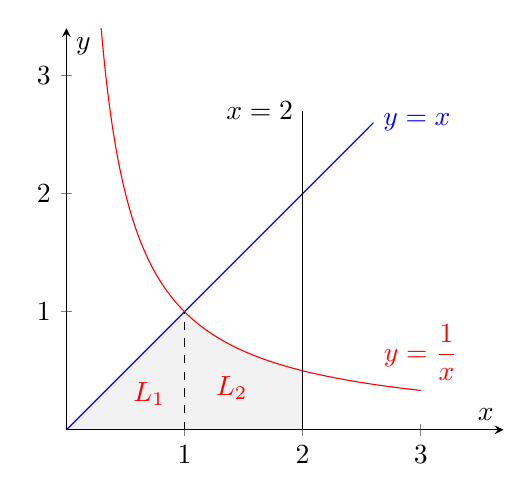
\begin{tikzpicture}
\begin{axis}[
x =1.5 cm, y=1.5 cm,
 axis lines=middle,
  xmin=0,xmax=3.7,ymin=0,ymax=3.4,
  xtick distance=1,
  ytick distance=1,
  xlabel=$x$,
  ylabel=$y$]
\addplot [blue,domain=0:1, name path=B] {x};
\addplot [blue,domain=1:2.6] {x} node[right] {$y=x$};
\addplot [red,domain=1:2, samples=1000, name path=A] {1/x};
\addplot [red,domain=0.1:1, samples=1000] {1/x};
\addplot [red,domain=2:3,samples=1000] {1/x} node[above] {$y=\dfrac{1}{x}$};
\addplot [domain=1:2, name path=C] {0};
\addplot [domain=0:1, name path=D] {0};
\addplot[gray,opacity=0.1] fill between[of=C and A];
\addplot[gray,opacity=0.1] fill between[of=B and D];
\draw (2,0) -- (2,2.7) node[left] {$x=2$};
\draw[dashed] (1,0) -- (1,1);
\draw[red] (0.7,0.3) node {$L_1$};
\draw[red] (1.4,0.35) node {$L_2$};
\end{axis}
\end{tikzpicture}
		\end{center}
		Luasnya dapat dibagi menjadi dua daerah seperti pada gambar, dengan batas dari $x=0$ sampai $x=1$ dan $x=1$ sampai $x=2$, sehingga
		\begin{align*}
		L = L_1 + L_2 &= \int_0^1 x \, dx +\int_1^2 \dfrac{1}{x} \, dx\\
		&= \dfrac{x^2}{2}\bigg|^1_0 + \ln x|^2_1\\
		&= \dfrac{1}{2} + \ln 2-\ln 1
		\end{align*}
Jadi luasnya adalah $\dfrac{1}{2}+\ln 2$ satuan luas.
	\item Tentukan volume dari benda padat yang terjadi bila daerah yang dibatasi oleh kurva $y=x, y=x^2$ diputar terhadap $x=2$.\\
	\textbf{Solusi:}\\
	\textbf{Metode Cakram}\\
	Tinjau bahwa kedua kurva berpotongan pada $(0,0)$ dan $(1,1)$ sehingga sketsanya 
	\begin{center}
		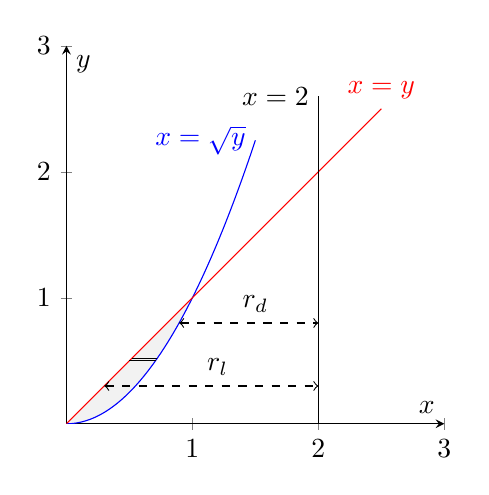
\begin{tikzpicture}
\begin{axis}[
x =1.6 cm, y=1.6 cm,
 axis lines=middle,
  xmin=0,xmax=3,ymin=0,ymax=3,
  xtick distance=1,
  ytick distance=1,
  xlabel=$x$,
  ylabel=$y$]
\addplot [blue, domain=0:1, samples=1000, name path=B] {x^2};
\addplot [blue, domain=1:1.5,samples=1000] {x^2} node[left] {$x=\sqrt{y}$};
\addplot [red, domain=0:1, name path=A] {x};
\addplot [red, domain=1:2.5] {x} node[above] {$x=y$};
\addplot[gray,opacity=0.1] fill between[of=B and A];
\draw (2,0) -- (2,2.6) node[left] {$x=2$};
\draw (0.707106,0.5) -- (0.5,0.5);
\draw (0.72111,0.52) -- (0.52,0.52);
\draw[dashed,<->] (0.3,0.3) -- (2,0.3);
\draw[dashed,<->] (0.8944271,0.8) -- (2,0.8);
\draw (1.2,0.45) node {$r_l$};
\draw (1.5,0.95) node {$r_d$};
\end{axis}
\end{tikzpicture}
		\end{center}
		Perhatikan bahwa untuk $x>0$, $x=\sqrt{y}$ dan $x=y$.\\
		Jari-jari dalamnya adalah $r_d=2-\sqrt{y}$ dan jari-jari luar adalah $r_l=2-y$. Perhatikan pula batasnya dari $y=0$ hingga $y=1$, maka
		\begin{align*}
		V = \pi \int_a^b r_l^2-r_d^2\, dy &= \pi \int_0^1 (2-y)^2-(2-\sqrt{y})^2\, dy\\
		&= \pi \int_0^1 4-4y+y^2-4+4\sqrt{y}-y\, dy\\
		&= \pi \int_0^1 y^2+4\sqrt{y}-5y\, dy\\
		&= \pi \left[\dfrac{y^3}{3}+\dfrac{8y\sqrt{y}}{3}-\dfrac{5y^2}{2}\right]^1_0\\
		&= \pi \left[\dfrac{1}{3}+\dfrac{8}{3}-\dfrac{5}{2}\right]\\
		&= \dfrac{\pi}{2}
		\end{align*}
	\textbf{Metode Cincin Silinder}\\
	Tinjau bahwa jari-jarinya adalah $r=2-x$ sedangkan tingginya $h=x-x^2$.
	\begin{center}
		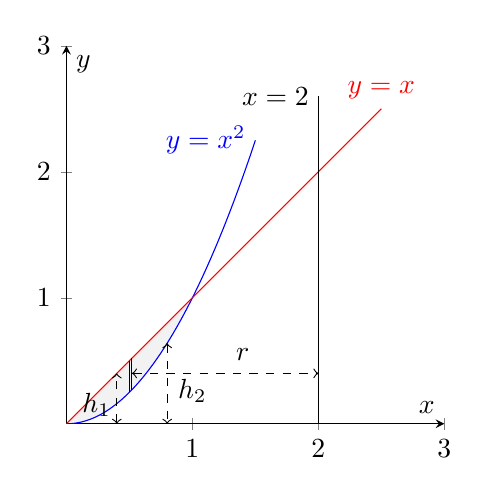
\begin{tikzpicture}
\begin{axis}[
x =1.6 cm, y=1.6 cm,
 axis lines=middle,
  xmin=0,xmax=3,ymin=0,ymax=3,
  xtick distance=1,
  ytick distance=1,
  xlabel=$x$,
  ylabel=$y$]
\addplot [blue, domain=0:1, samples=1000, name path=B] {x^2};
\addplot [blue, domain=1:1.5,samples=1000] {x^2} node[left] {$y=x^2$};
\addplot [red, domain=0:1, name path=A] {x};
\addplot [red, domain=1:2.5] {x} node[above] {$y=x$};
\addplot[gray,opacity=0.1] fill between[of=B and A];
\draw (2,0) -- (2,2.6) node[left] {$x=2$};
\draw (0.5,0.25) -- (0.5,0.5);
\draw (0.52,0.52*0.52) -- (0.52,0.52);
\draw[dashed,<->] (0.4,0) -- (0.4,0.4);
\draw[dashed,<->] (0.8,0.8*0.8) -- (0.8,0);
\draw (0.24,0.15) node {$h_1$};
\draw (1,0.26) node {$h_2$};
\draw[dashed,<->] (0.52,0.4) -- (2,0.4);
\draw (1.4,0.55) node {$r$};
\end{axis}
\end{tikzpicture}
		\end{center}
		Perhatikan bahwa batasnya dari $x=0$ hingga $x=1$ sehingga diperoleh
		\begin{align*}
		V = 2\pi\int_a^b rh \, dx &= 2\pi \int_0^1 (2-x)(x-x^2)\, dx\\
		&= 2\pi \int_0^1 2x-3x^2+x^3 \, dx\\
		&= 2\pi \left[x^2-x^3+\dfrac{1}{4}x^4\right]^1_0\\
		&= 2\pi \left[1-1+\dfrac{1}{4}\right]\\
		&= \dfrac{\pi}{2}
		\end{align*}
		Jadi volumenya adalah $\dfrac{\pi}{2}$ satuan volume.
\end{enumerate}
\newpage
\section*{SOAL KELAS 53-61}
\begin{enumerate}
	\item Diberikan bahwa untuk $x>0,x\neq 1,$ dan $y\neq 1$
	$$ \log_x y = \log_y x \qquad \text{dan}\qquad \log_x(x-y) = \log_y(x+y)$$
	Tunjukkan bahwa $x^4-x^2-1=0$\\
	\textbf{Solusi:}\\
	Perhatikan bahwa
	\begin{align*}
	\log_x y = \dfrac{1}{\log_y x} &= \log_y x\\
	\log_y^2 (x)-1 &= 0\\
	(\log_y (x)-1)(\log_y (x)+1) &= 0\\
	\log_y (x) &= \pm 1\\
	y = x \vee \dfrac{1}{y} &= x
	\end{align*}
	Jika $x=y$, maka $x-y=0$ sehingga tidak memenuhi syarat domain pada persamaan kedua. Jadi $x=\dfrac{1}{y}$, sehingga
	\begin{align*}
	\log_x \left(x-\dfrac{1}{x}\right) &= \log_{\frac{1}{x}} \left(x+\dfrac{1}{x}\right)\\
	\log_x \left(x-\dfrac{1}{x}\right) &= -\log_{x} \left(x+\dfrac{1}{x}\right)\\
	\log_x \left(x-\dfrac{1}{x}\right) +\log_{x} \left(x+\dfrac{1}{x}\right) &= 0\\
	\log_x \left[\left(x-\dfrac{1}{x}\right)\left(x+\dfrac{1}{x}\right)\right] &= 0\\
	\log_x \left(x^2-\dfrac{1}{x^2}\right) &= 0\\
	x^0 = 1 &= x^2-\dfrac{1}{x^2}
	\end{align*}
	Diperoleh $x^4-1 = x^2$ sehingga $x^4-x^2-1=0$. Terbukti.
	\item Selesaikan 
	$$ \int \dfrac{x^4+2}{x^3+9x}\, dx$$
	\textbf{Solusi:}\\
	Tinjau bahwa $	x^4+2 = x^2(x^2+9)-9x^2+2 $. Selanjutnya akan dicari dekomposisi dari $\dfrac{-9x^2+2}{x^3+9x}$, yaitu
	\begin{align*}
	\dfrac{-9x^2+2}{x(x^2+9)} &= \dfrac{A}{x} + \dfrac{Bx+C}{x^2+9}\\
	&= \dfrac{(A+B)x^2+Cx+9A}{x^3+9x}
	\end{align*}
	Diperoleh 
	$$ A+B = -9 \qquad\text{dan}\qquad C=0\qquad\text{dan}\qquad 9A=2$$
	Jadi $A=\dfrac{2}{9}$, $B=-\dfrac{83}{9},$ dan $C=0$, maka
	\begin{align*}
	\int \dfrac{x^4+2}{x^3+9x}\, dx &= \int \dfrac{x^2(x^2+9)-9(x^2+9)+83}{x(x^2+9)}\, dx\\
	&= \int x + \dfrac{2}{9x} -\dfrac{83x}{9(x^2+9)}\, dx\\
	&= \dfrac{x^2}{2}+\dfrac{2}{9}\ln x-\dfrac{83}{18}\ln(x^2+9) + C
	\end{align*}
	\item Dapatkan nilai integral berikut ini jika konvergen:
	$$ \int_{-3/2}^0 \dfrac{x+2}{\sqrt{2x+3}}\, dx$$
	\textbf{Solusi:}\\
	Misalkan $2x+3=u$ sehingga $2\, dx=du$. Untuk $x=-\dfrac{3}{2}$, maka $u=0$, dan untuk $x=0$, maka $u=3$. Diperoleh pula $x=\dfrac{u-3}{2}$ sehingga $x+2=\dfrac{u+1}{2}$. Jadi diperoleh 
	\begin{align*}
	\int_{-3/2}^0 \dfrac{x+2}{\sqrt{2x+3}}\, dx &= \int_0^3 \dfrac{u+1}{4\sqrt{u}} \, du\\
	&= \lim_{a\rightarrow 0^+} \dfrac{1}{4}\int_a^3 \sqrt{u} + u^{-\frac{1}{2}} \, du\\
	&= \lim_{a\rightarrow 0^+} \dfrac{1}{4}\left[\dfrac{2u\sqrt{u}}{3}+2\sqrt{u}\right]^3_a\\
	&= \lim_{a\rightarrow 0^+} \dfrac{1}{4}\left[2\sqrt{3}+2\sqrt{3} - \dfrac{2a\sqrt{a}}{3}-2\sqrt{a}\right] = \sqrt{3}
	\end{align*}
	\item Hitung $$ \lim_{x\rightarrow 0^+} (\sin x)^{\sqrt{x}} $$
	\textbf{Solusi:}\\
	\textbf{Cara I}\\
	Tinjau bahwa $(\sin x)^{\sqrt{x}}=e^{\ln(\sin x)^{\sqrt{x}}}=e^{\sqrt{x}\ln(\sin x)}=e^{\frac{\ln(\sin x)}{1/\sqrt{x}}}$. Dari sini diperoleh bentuk tak tentu, sehingga dapat digunakan aturan L'Hopital
	\begin{align*}
	\lim_{x\rightarrow 0^+} \frac{\ln(\sin x)}{1/\sqrt{x}} &= \lim_{x\rightarrow 0^+} \dfrac{\frac{1}{\sin x}\cos x}{-\frac{1}{2x\sqrt{x}}}\\
	&= \lim_{x\rightarrow 0^+} -\dfrac{2x\sqrt{x}}{\tan x}\\
	&= \lim_{x\rightarrow 0^+} \dfrac{x}{\tan x}\times \lim_{x\rightarrow 0^+} (-2x)\\
	&= 1\times 0 = 0 
	\end{align*}
	Jadi $$ \lim_{x\rightarrow 0^+} (\sin x)^{\sqrt{x}} = \lim_{x\rightarrow 0^+} e^{\frac{\ln(\sin x)}{1/\sqrt{x}}} = e^{\left(\lim_{x\rightarrow 0^+}\frac{\ln(\sin x)}{1/\sqrt{x}}\right)} = e^0 = 1 $$
	\textbf{Cara II}\\
	Perhatikan bahwa $-1\leq \sin x\leq 1$ sehingga $(-1)^{\sqrt{x}}\leq (\sin x)^{\sqrt{x}} \leq 1^{\sqrt{x}}$, akibatnya 
	\begin{align*}
	1=\lim_{x\rightarrow 0^+} (-1)^{\sqrt{x}} \leq \lim_{x\rightarrow 0^+}(\sin x)^{\sqrt{x}} \leq \lim_{x\rightarrow 0^+} 1^{\sqrt{x}} = 1
	\end{align*}
	Dengan teorema apit, didapatkan $\displaystyle \lim_{x\rightarrow 0^+}(\sin x)^{\sqrt{x}}=1$
	\item Diberikan $R$ adalah daerah yang dibatasi oleh sumbu $x$, kurva $y=e^{-x}$, dan sumbu $y$. Jika $R$ diputar terhadap sumbu $x$, tentukan volume benda pejal yang dihasilkan.\\
	\textbf{Solusi:}\\
	Dalam pembahasan ini, digunakan metode cakram, karena jika menggunakan metode cincin silinder, integralnya akan lebih sulit untuk dihitung.\\
	Tinjau bahwa jari-jarinya $r_l=e^{-x}$ dan $r_d=0$. Batas integralnya dari $x=0$ sampai $x$ menuju tak hingga
	\begin{center}
		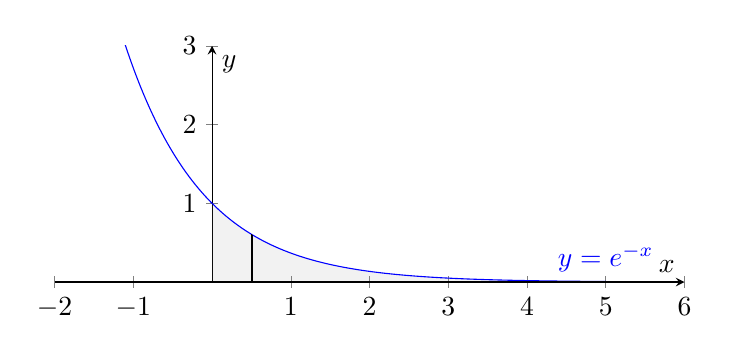
\begin{tikzpicture}
\begin{axis}[
x =1 cm, y=1 cm,
 axis lines=middle,
  xmin=-2,xmax=6,ymin=0,ymax=3,
  xtick distance=1,
  ytick distance=1,
  xlabel=$x$,
  ylabel=$y$]
\addplot [blue,domain=0:5, samples=1000, name path=B] {exp(-x)} node[above] {$y=e^{-x}$};
\addplot [blue,domain=-2:0, samples=1000] {exp(-x)};
\addplot [domain=0:5, name path=A] {0};
\addplot[gray,opacity=0.1] fill between[of=B and A];
\draw (0.5, 0.606531) -- (0.5,0);
\draw (0.51, 0.600496) -- (0.51,0);
\end{axis}
\end{tikzpicture}
		\end{center}
		Diperoleh 
		\begin{align*}
		V = \pi \int_a^b r_l^2 - r_d^2 \, dx &= \pi \int_0^{\infty} e^{-2x} \, dx\\
		&= \pi \lim_{a\rightarrow \infty} \int_0^a e^{-2x} \, dx\\
		&= \pi \lim_{a\rightarrow \infty} -\dfrac{1}{2e^{2x}} \bigg|^a_0\\
		&= \pi \lim_{a\rightarrow \infty} \left(-\dfrac{1}{2e^{2a}}+\dfrac{1}{2}\right)\\
		&= \dfrac{\pi}{2}
		\end{align*}
		Jadi volume benda putar yang terjadi adalah $V=\dfrac{\pi}{2}$
\end{enumerate}
\newpage
\section*{SOAL KELAS 62-70}
\begin{enumerate}
	\item \begin{enumerate}
		\item Dapatkan penyelesaian dari persamaan $\ln(e^{-x}-1)=x$
		\item Dapatkan $\dfrac{dy}{dx}$ dari $y=\ln(\cosh^{-1}x)$
	\end{enumerate}
	\textbf{Solusi:}
	\begin{enumerate}
		\item Tinjau bahwa 
		\begin{align*}
		e^x &= e^{-x}-1\\
		e^{2x} &= 1-e^x\\
		e^{2x}+e^x-1 &= 0 \\
		e^x &= \dfrac{-1\pm \sqrt{1^2-4(1)(-1)}}{2(1)} \\
		&= \dfrac{-1\pm\sqrt{5}}{2}
		\end{align*}
		Karena $e^x>0$, maka $e^x=\dfrac{-1+\sqrt{5}}{2}$ sehingga $x=\ln \left(\dfrac{-1+\sqrt{5}}{2}\right)$
		\item Ingat kembali aturan rantai, turunan dari $\ln x$ dan $\cosh^{-1}x$, diperoleh 
		\begin{align*}
		\dfrac{dy}{dx}\ln(\cosh^{-1}x) &= \dfrac{1}{\cosh^{-1}x}\times \dfrac{1}{\sqrt{x^2-1}}\\
		&= \dfrac{1}{(\cosh^{-1}x)\sqrt{x^2-1}}
		\end{align*}
	\end{enumerate}
	\item Diberikan $\theta=\sin^{-1}\left(-\dfrac{1}{2}\sqrt{3}\right)$. Tentukan nilai eksak dari: $\cos\theta,\tan\theta,$ dan $\cot\theta$.\\
	\textbf{Solusi:}\\
	Dapat diperoleh bahwa $\sin\theta=-\dfrac{1}{2}\sqrt{3}$ dengan $-\dfrac{\pi}{2}\leq\theta\leq\dfrac{\pi}{2}$ sehingga $\theta$ yang memenuhi adalah $-\dfrac{\pi}{3}$. Jadi dapat diperoleh 
	\begin{align*}
	\cos\theta &= \cos \left(-\frac{\pi}{3}\right) = \dfrac{1}{2}\\
	\tan\theta &= \tan \left(-\frac{\pi}{3}\right) = -\sqrt{3}\\
	\cot\theta &= \cot \left(-\frac{\pi}{3}\right) = -\dfrac{1}{3}\sqrt{3}
	\end{align*}
	\newpage
	\item Selesaikan
	$$ \int \dfrac{4x-1}{2x^3-x^2}\, dx $$
	\textbf{Solusi:}\\
	Tinjau bahwa $2x^3-x^2=x^2(2x-1)$ sehingga dekomposisi pecahannya adalah 
	\begin{align*}
	\dfrac{4x-1}{2x^3-x^2} &= \dfrac{A}{x}+\dfrac{B}{x^2} + \dfrac{C}{2x-1}\\
	&= \dfrac{Ax+B}{x^2}+\dfrac{C}{2x-1}\\
	&= \dfrac{(Ax+B)(2x-1)+Cx^2}{x^2(2x-1)}\\
	&= \dfrac{2Ax^2+2Bx-Ax-B+Cx^2}{x^2(2x-1)}\\
	&= \dfrac{(2A+C)x^2+(2B-A)x-B}{x^2(2x-1)}
	\end{align*}
	Dapat diperoleh bahwa 
	\begin{align*}
	2A+C &= 0\\
	2B-A &= 4\\
	-B &= -1
	\end{align*}
	Kita dapatkan $A=-2,B=1,C=4$ sehingga
	\begin{align*}
	\int \dfrac{4x-1}{2x^3-x^2}\, dx &= \int -\dfrac{2}{x}+\dfrac{1}{x^2}+\dfrac{4}{2x-1}\\
	&= -2\ln|x| - \dfrac{1}{x} + 2\ln|2x-1| +C
	\end{align*}
	\item Selesaikan integral dari $$\int_{-\infty}^{\infty}\dfrac{e^{-t}}{1+e^{-2t}}\, dt$$
	\textbf{Solusi:}\\
	Misalkan $e^{-t}=u$ sehingga $-e^{-t}\, dt=du$. Untuk $t\rightarrow -\infty$, maka $u\rightarrow +\infty$ dan untuk $t\rightarrow \infty$, maka $u\rightarrow 0$
	\begin{align*}
	\int_{-\infty}^{\infty}\dfrac{e^{-t}}{1+e^{-2t}}\, dt &= \int_{+\infty}^{0}-\dfrac{1}{1+u^2}\, du \\
	&= \int_0^{+\infty} \dfrac{1}{1+u^2}\, du\\
	&= \lim_{a\rightarrow +\infty}\int_0^a \dfrac{1}{1+u^2}\, du\\
	&= \lim_{a\rightarrow +\infty} \tan^{-1}(u)\bigg|^a_0\\
	&= \lim_{a\rightarrow +\infty} \tan^{-1}(a)-\tan^{-1}(0)\\
	&= \lim_{a\rightarrow +\infty} \tan^{-1}(a)-0
	\end{align*}
	Tinjau bahwa $\displaystyle \lim_{a\rightarrow +\infty} \tan^{-1}(a)=\dfrac{\pi}{2}$ sehingga 
	$$ \int_{-\infty}^{\infty}\dfrac{e^{-t}}{1+e^{-2t}}\, dt = \dfrac{\pi}{2}$$
	\item Dapatkan volume benda putar yang terjadi jika dataran yang dibatasi oleh kurva $x=9-y^2$ dan $x-y-7=0$, diputar terhadap garis $y=A$, di mana $A$ adalah digit terakhir NRP anda. Jika digit terakhir adalah 0 maka ganti dengan 10 (sertai dengan gambar)\\
	\textbf{Solusi:}\\
	Tinjau bahwa $x=y+7$ sehingga titik potongnya adalah
	\begin{align*}
	y+7 &=9-y^2\\
	y^2+y-2 &= 0\\
	(y+2)(y-1) &=0
	\end{align*}
	Untuk $y=-2$, maka $x=5$, dan untuk $y=1$, maka $x=8$. Diperoleh titik potongnya adalah $(5,-2)$ dan $(8,1)$. Berikut grafiknya
	\begin{center}
		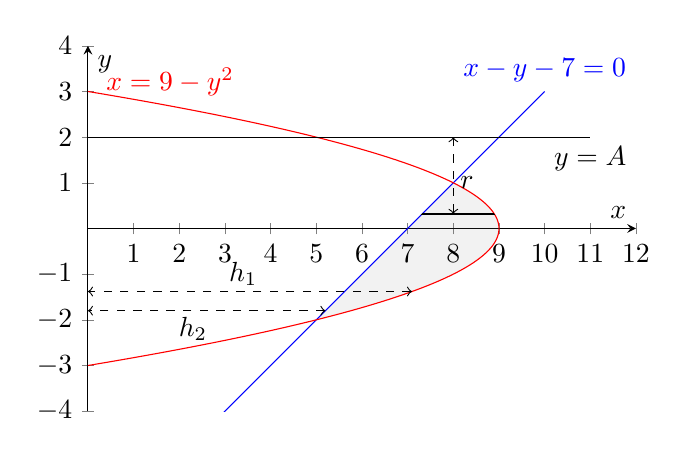
\begin{tikzpicture}
\begin{axis}[
x =.58 cm, y=.58 cm,
 axis lines=middle,
  xmin=0,xmax=12,ymin=-4,ymax=4,
  xtick distance=1,
  ytick distance=1,
  xlabel=$x$,
  ylabel=$y$]
\addplot [blue,domain=5:8, samples=1000, name path=B] {x-7};
\addplot [blue,domain=0:5] {x-7};
\addplot [blue,domain=8:10] {x-7} node[above] {$x-y-7=0$};
\addplot [red,domain=8:9, samples=1000,name path=A] {sqrt(9-x)};
\addplot [red,domain=0:8, samples=1000] {sqrt(9-x)};
\addplot [red,domain=8:9, samples=1000,name path=D] {-sqrt(9-x)};
\addplot [red,domain=5:8, samples=1000,name path=C] {-sqrt(9-x)};
\addplot [red,domain=0:5, samples=1000] {-sqrt(9-x)};
\addplot [domain=0:11] {2} node[below] {$y=A$};
\draw (7.3,0.3) -- (9-0.3^2,0.3);
\draw (7.32,0.32) -- (9-0.32^2,0.32);
\draw[<->,dashed] (8,0.32) -- (8,2);
\draw (8.3,1) node {$r$};
\addplot[gray,opacity=0.1] fill between[of=B and C];
\addplot[gray,opacity=0.1] fill between[of=A and D];
\draw[dashed,<->] (-1.8+7,-1.8) -- (0,-1.8);
\draw[dashed,<->] (9-1.38^2,-1.38) -- (0,-1.38);
\draw (2.3,-2.2) node {$h_2$};
\draw (3.4,-1) node {$h_1$};
\draw[red] (1.8,3.2) node {$x=9-y^2$};
\end{axis}
\end{tikzpicture}
		\end{center}
		Perhatikan bahwa jika kita gunakan metode cakram, maka kita perlu membagi daerah integrasi menjadi dua bagian, yaitu untuk $5\leq x\leq 8$ dan $8\leq x\leq 9$, karena batas "atas" fungsinya berbeda. Oleh karena itu, gunakan metode cincin silinder supaya lebih mudah. \\
		Tinjau bahwa $1\leq A\leq 10,~ A\in \mathbb{N}$, sehingga titik perpotongan "atas" kedua kurva berada pada garis $y=A$ atau di bawahnya, maka jari-jarinya $r=A-y$ dan tingginya $h=9-y^2-(y+7)=-y^2-y+2$. Batasnya adalah dari $y=-2$ sampai $y=1$
		\begin{align*}
		V = 2\pi \int_a^b rh \, dy &= 2\pi \int_{-2}^1 (A-y)(-y^2-y+2) \, dy\\
		&= 2\pi \int_{-2}^1 y^3 +(1-A)y^2-(2+A)y+2A\, dy\\
		&= 2\pi \left[\dfrac{y^4}{4}+\dfrac{1-A}{3}y^3-\dfrac{2+A}{2}y^2+2Ay\right]^1_{-2}\\
		&= 2\pi\left[\left(\dfrac{1}{4}+\dfrac{1-A}{3}-\dfrac{2+A}{2}+2A\right)-\left(4-\dfrac{8(1-A)}{3}-2(2+A)-4A\right)\right]\\
		&= \dfrac{18A+9}{2}\pi
		\end{align*}
\end{enumerate}
\end{document}
